%===============================================================================================
%		Requirements
%===============================================================================================

\part{Requirements}
\label{sec:Analyse}

This chapter defines the most important functional and non-functional requirements for \LibName{}.
Most relevant input is the document \cite{MC17}.

%===============================================================================================
%		Scope
%===============================================================================================

\chapter{Scope}


% -------------------------------------------------------------------------------------------------------
%  In Scope
% -------------------------------------------------------------------------------------------------------
\section{In Scope}%
\label{sec:InScope}%

\LibName{} is a Java library for reading and writing container and metadata formats. \LibName{} has the following goals:
\begin{itemize}
\item Define a robust, easy to use and generic API for reading and writing multimedia (i.e. audio, video and image) metadata
\item In addition, define a way to also parse and change typical container formats that embed or surround multimedia metadata
\item Be easily extensible with additional metadata or container formats, also by third party
\end{itemize}

Thus, clearly, \LibName{} targets applications and users in the multimedia editing area, e.g. software to manage an audio, video or image collection.

Special strenght of the library should be its versatility (in a sense of supported formats and generality) as well as its extensibility. At the same time, it targets to offer access to ALL features of each specific format, even the low-level ones, and thus does not want to hide anything from expert users who need fine-grained control.

Using \LibName{}, an application is allowed to access metadata quite generically and comfortably, or it can also explore deep specifics of each format down to the bit and byte level.

% -------------------------------------------------------------------------------------------------------
%  Out of Scope
% -------------------------------------------------------------------------------------------------------
\section{Out of Scope}%
\label{sec:OutofScope}%

Metadata not in the audio, video or image domain are not directly in scope of \LibName{} and thus the library might not offer the right abstractions for those. However, it is at least likely that other binary or textual formats can also be parsed quite the same way using \LibName{}.

Furthermore, \LibName{} clearly is no encoding or decoding library, it cannot understand codecs. It might however help to encode or decode by providing access to the low-level details of the container formats. It might be used as basis for extensible encoders or decoders, however, not exactly in high-performance areas where speed is of most importance. 

Further things out of scope of specific versions are treated in \SectionLink{sec:Requirements}.

%-----------------------------------------------------------------------------------------------
%		Features of version \LibVersion{}
%-----------------------------------------------------------------------------------------------

\section{Features of version \LibVersion{}}
\label{sec:FeaturesLibVersion}

Here we give a brief overview of the features the library needs to offer in version \LibVersion{}. It is the first version of the library, so its goal is the bare minimum: Implement all core features and support some of the most important data formats. Image and video formats are not yet in scope of this version. 

%-----------------------------------------------------------------------------------------------

\subsection{Supported Platforms}
\label{sec:SupportedPlatforms}

In general, \LibName{} in its current version \LibVersion{} can be used with any platform that also supports Java SE in \JavaVersion{}. However, it needs to be specified for which platforms tests were run explicitly and thus it is proven that specific features work on these platforms. We target to support the following platforms like this:
\begin{itemize}
\item Windows 10
\item Ubuntu 16.04
\end{itemize}

%-----------------------------------------------------------------------------------------------

\subsection{Supported Metadata Formats}
\label{sec:UnterstuetzteMetadatenformate}

This version adds support for the following audio metadata formats:

\begin{itemize}
\item ID3v1 and ID3v1.1
\item ID3v2.3
\item APEv2
\item Lyrics3v2
\end{itemize}

%-----------------------------------------------------------------------------------------------

\subsection{Supported Container Formate}
\label{sec:UnterstuetzteContainerformate}

This version adds support for the following audio container formats:

\begin{itemize}
\item MPEG-1 Audio Layer 3 (MP3)
\end{itemize}

%-----------------------------------------------------------------------------------------------

\subsection{Supported Input Media}
\label{sec:UnterstuetzteEingabemedien}

This version adds support for the following data sources for reading data:
\begin{itemize}
\item Files
\item Java \texttt{InputStream}s
\item Java byte arrays
\end{itemize}

%-----------------------------------------------------------------------------------------------

\subsection{Supported Output Media}
\label{sec:UnterstuetzteAusgabemedien}

This version adds support for the following output media for writing data:
\begin{itemize}
\item Files
\item Java byte arrays
\end{itemize}

%-----------------------------------------------------------------------------------------------
%		Related Libraries
%-----------------------------------------------------------------------------------------------

\section{Related Libraries}
\label{sec:RelatedLibraries}

Here, related Java libraries are treated that are related to what \LibName{} offers. This includes existing productive Java libraries in the area of multimedia, which can be considered as open source competitors to \LibName{} on the one hand, on the other hand, they provide inspiration, possible reuse and also warning examples how to not do it.

%-----------------------------------------------------------------------------------------------

\subsection{Metadata Libraries}
\label{sec:MetadataLibraries}

A selection of libraries offering access to multimedia metadata as of end of 2017, mostly audio metadata - One source for this e.g. is \url{http://id3.org/Implementations} and Google:

\begin{landscape}
\begin{longtable}{|p{0.18\linewidth}|p{0.22\linewidth}|p{0.18\linewidth}|p{0.07\linewidth}|p{0.25\linewidth}|}
	\hline
	\rowcolor[gray]{.9}\textbf{Library} & \textbf{URL} & \textbf{Supported Formats} & \textbf{Lines of Code} & \textbf{Comments} \\
	\endhead
	\hline
\textbf{jaudiotagger (Java)} & \url{http://www.jthink.net/jaudiotagger/} &  MP3, MP4, Ogg Vorbis, Flac, WMA, partly WAV and Real Audio & $>86000$ & Obscure class and package structure, more than 500 classes, just a few testcases only (?), still actively developed \\
	\hline
\textbf{jLayer and JavaZoom (Java)} & \url{http://www.javazoom.net/index.shtml} & MP3, WAV, ID3v1, ID3v2 & $>13600$ & Project targeting MP3 decoding and playing of MP3s \\
	\hline
\textbf{mp3agic (Java)} & \url{https://github.com/mpatric/mp3agic} & ID3 Tags (1.0, 1.1, 2.3, 2.4), Read-only ID3 v2.2, MP3 low-level reading (incl. VBR) & $>5500$ & Still actively developed \\
	\hline
\textbf{BeagleBuddy (Java)} & \url{http://www.beaglebuddy.com/} & Reads and writes ID3 Tags (1.0, 1.1, 2.3, 2.4), Lyrics3v2, Lyrics3v1, APEv1, APEv2, reads MP3 files CBR and VBR, Xing, LAME, and VBRI Header & $>40700$ & Focus on being ``easy to use''; Last version in beginning of 2015 \\
	\hline
\textbf{JID3 (Java)} & \url{https://blinkenlights.org/jid3/}, \url{https://java.net/projects/jid3lib} & ID3v1, ID3v2.2 and ID3v2.3; no ID3v2.4 support & $>30000$ & Seems to be dead (last version 0.46 in 2005) \\
 	\hline
\textbf{Javamusictag (Java)} & \url{http://javamusictag.sourceforge.net/} & MP3, ID3v1, ID3v1.1, Lyrics3v1, Lyrics3v2, ID3v2.2, ID3v2.3, and ID3v2.4 & $>27000$ & Seems to be the same thing or a fork of JID3 \\
 	\hline
\textbf{Xuggler (Java)} & \url{http://www.xuggle.com/xuggler} & MP3, Ogg (Vorbis, Speex), Flac, AAC, ID3v2 and others & - & Decoder and editing API for various audio and video formats \\
	\hline
\textbf{jFlac (Java)} & \url{http://jflac.sourceforge.net/} & FLAC, VorbisComment & 13000 & Especially encoding and decoding of FLAC \\
	\hline
\textbf{MPEG-7 Audio Encoder (Java)} & \url{http://mpeg7audioenc.sourceforge.net/} & MPEG-7 & - & Creates MPEG-7 metadata \\
	\hline
\textbf{JAI Image I/O (Java)} & \url{https://jai-imageio.dev.java.net/binary-builds.html} & EXIF & - & Can read and write EXIF tags from a variety of embedding formats \\
	\hline
\textbf{jmac (Java)} & \url{http://sourceforge.net/projects/jmac/} & APE, MonkeyAudio & - & \\
	\hline
 \textbf{MyID3 (Java)} & \url{https://github.com/jkauflin/jjkMP3} & Audio-Metadaten (ID3) & - & Private engagement, not really to be taken seriously \\
	\hline
\textbf{id3lib (C/C++)} & \url{http://id3lib.sourceforge.net/} & Audio-Metadaten (ID3) & - & \\
	\hline
\textbf{Mutagen (Python)} & \url{http://pypi.python.org/pypi/mutagen/1.12} & Audio-Metadaten und -Container-Daten (ID3) & & \\
	\hline
\caption{Competitor libraries compared}
\label{tab:Compet}
\end{longtable}
\end{landscape}

The analysis shows that as of now, the biggest competitors would be jAudioTagger, mp3agic, BeagleBuddy and JID (which seems dead) from a metadata perspective and Xuggler as well as jLayer from decoding and editing perspective (if \LibName{} should ever try to go into this direction).

%***********************************************************************************************

\subsubsection{Drawbacks of Existing Metadata Libraries}
\label{sec:DrawbacksofExistingMetadataLibraries}

Each of the mentioned libraries specializes itself to just a few formats. Saying this, applications are only likely to be satisfied with them if they just need to support those formats. If they do require more, they need to use multiple libraries or extend the existing ones or wait for new features.

Second, the architecture and extensibility of the existing libraries is not convincing. Most of the ID3 libraries e.g. open-heartedly show their very internals, which does not make it clear what really distinguishes ``public API'' and the private parts - with the usual consequences. Users might rely on private implementation aspects that are changed later, or if it is known that users do so for specific parts, the library evolution might get constrained by this, forcing duplication and maintenance of actually obsolete code.

Another smell of most of the libraries is their sheer volume: While mp3agic still seems humble in terms of ``only'' about 6000 lines of code (including comments and blank lines), it also does not offer so much features. The other libraries can really be considered big, topping to about over 86000 lines of code for jaudiotagger. These libraries also do not show an obvious structure or core concepts springing to one's eyes. Maintainability and especially extensibility of such rather ``hardcoded'' libraries might be not too easy.    

Users / software needing to support a broad variety of formats - when using these formats - likely need to implement a kind of plugin mechanism for easier extensibility themselves.

%***********************************************************************************************

\subsubsection{Advantages of \LibName{}}
\label{sec:AdvantagesofLibName}

There are alreads so much library - why do we need \LibName{}? If it wants to do things better, a lot of effort is required. Is that worth it?

There are multiple aspects where \LibName{} can do better than existing libraries:
\begin{itemize}
\item \LibName{} should target container formats on a very abstract and generic level, yet still providing access to the bare details of each format; this can go as far as providing a generic framework for parsing and writing any multimedia container format, may it be audio, video, image or text content.
\item Applications whose core asset is extensibility and rich variety of supported formats do not have to use a dozen or so third party libraries having completely different programming, license and support models as well as performance characteristics - provided \LibName{} actually offers support for all formats, which is of course not necessarily the case
\item However, at least such applications do not need to reinvent the wheel by coding their own extensibility mechanism, but they just rely on the extensibility mechanism by using \LibName{}; they can code their own \LibName{} extension to support another format. The goal of \LibName{} is that doing so is easier for such applications than using another 3rd party library to enable support for such a format.
\item Still, \LibName{} is not a huge Uber JAR containing all supported formats, but it is modular, where applications just need the core of the library plus an extension module per format they want to support.
\item \LibName{} also targets to offer an easy to learn and use API for such applications.
\end{itemize}

All that said, the benchmark for how good \LibName{} really is, is as follows:
\begin{itemize}
\item It should be easier to use as BeaglyBuddy which claims to be easy to use
\item It should be much less complex (means to say: much less classes and lines of code) than jaudiotagger or BeagleBuddy
\item Supporting a new, averagely complex, previously unsupported data format does not take an experienced Java programmer (who never did write a \LibName{} extension) more than one man day!
\item Likewise, we also want to compete with other libraries in terms of performance: \LibName{} must at least be comparatively fast as the most important competitors for Java, ideally of course it should be faster
\end{itemize}

%-----------------------------------------------------------------------------------------------

\subsection{Multimedia Libraries}
\label{sec:MultimediaLibraries}

Can \LibName{} cooperate, i.e. reuse or integrate with existing Java multimedia libraries? This question is not really answered in the following sections. The general answer is: No, \LibName{} will neither be some kind of plugin for the existing libraries, nor will it depend on them, nor will it consider the requirement of easy cooperation or integration with this libraries in any way.

For now, we just want to see what is existing in the wild in terms of Java multimedia libraries, mostly audio and video. This evaluation might point future directions for \LibName{} if it goes to probably superseding or extending the existing options.

All or most of the multimedia libraries listed here seem to offer some way of reading or writing multimedia metadata. But mostly, these libraries focus on streaming, playing, encoding and decoding on high performance. The metadata is just a side-product that seems to be offered most of the time via a rather inconvenient API.

% -------------------------------------------------------------------------------------------------------
\subsubsection{Xuggler and Humble Video}%
\label{sec:Xuggler}%

Cite from the ebsite: ``Xuggler is the easy way to uncompress, modify, and re-compress any media file (or stream) from Java. ... Xuggler allows Java programs to decode, encode, and experience (almost) any video format.''

It does not seem to be based on GStreamer or FFMPEG or JMF. It does not become clear which formats are supported by the library.

The official Github page of Xuggler states it is outdated and humble video should be used. The name suggests Humble Video is mainly focused on video, not audio such as MP3.

% -------------------------------------------------------------------------------------------------------
\subsubsection{JLayer}%
\label{sec:JLayer}%

Cite for JLayer: ``JLayer is a JAVA library that decodes, converts and plays MP3 files in real-time. JLayer supports MPEG 1/2/2.5 Layer 1/2/3 audio format. JLayer doesn't need JMF.''

It does also not seem to rely on GStreamer or FFMPEG but seems to be a ``native'' Java only implementation for encoding and decoding MP3 audio data.

% -------------------------------------------------------------------------------------------------------
\subsubsection{Java FX and GStreamer}%
\label{sec:JavaFX}%

JavaFX is an Oracle library to support with platform-independent handling of user interfaces as well as multimedia content. So, it is not only ``GUI'' that actually replaces Swing and AWT, but also handling of images, video and audio content as well as even 3D graphics, thus somewhat replacing the obsolete Java 3D.

So it has a quite broad usage space. However, there is also some muttering that it might be dead or at least does not have a bright future.

For local GUIs it might still be a good option. What about multimedia playback, editing etc.? The media engine part of JavaFX is based on GStreamer. GStreamer is an extensive audio and video library written in C and nevertheless platform-independent by being ported to a lot of platforms and architectures. It also supports reading and writing tags, but in a very specific generic API which does not offer too much comfort. But how does this go together with JavaFX? First of all, GStreamer also offers a Java binding, i.e. can be called from Java applications where any installed GStreamer plugins for formats can also be used. This interface is most probably also used by JavaFX. JavaFX then offers a class named MediaPlayer with a method chain \texttt{getMedia().getMetadata()}, just returning a map (String to Object). There seems to be no documentation which objects might get returned. Furthermore it just seems to be read-only, there does not seem to be any way of writing tags with JavaFX.

% -------------------------------------------------------------------------------------------------------
\subsubsection{FFMPEG}%
\label{sec:FFMPEG}%

FFMPEG can be seen as direct competition to GStreamer, being a platform-independent framework and toolkit to record, convert and stream audio and video content. It is also written in C/C++ and supports a variety of formats. 

%***********************************************************************************************

\subsubsection{JMF and FMJ}
\label{sec:JMF}

The Java Media Framework is an official Java library that is delivered with J2SE \emph{desktop} technology. The most recent version is 2.1.1e and dating back to 2001. Which actually means: It is dead. However, we still consider it a bit here. JMF can be used by Client as well as server applications. JMF was packaged with an MP3 decoder and encoder until 2002, but removed due to licensing issues. Since 2004 there is an MP3 playback only plug-in.\footnote{see \cite{WikJMF}.}

FMJ is an Open Source Alternative, that is API compatible: \url{http://www.fmj-sf.net/}. But FMJ also seems to be dead.

JMF comes in four JAR files:\footnote{Siehe \cite{WikJMF}.}
\begin{itemize}
\item JMStudio: Simple multimedia player application
\item JMFRegistry: An application to manage different JMF settings and plug-ins
\item JMFCustomizer: Allows creation of a simple JMF JAR file containing only those JMF classes needed by the client application
\item JMFInit: Inititializes a JMF application
\end{itemize}

JMF contains platform-specific \emph{performance packs}, i.e. optimized packtes for Linux, Solaris or Windows.

%***********************************************************************************************

\paragraph{Features:}
\label{sec:Features}

JMF deals with time-based media. The JMF features can be summed up as follows:\footnote{Siehe \cite{JMFWeb}.}
\begin{itemize}
\item Capture: Read multimedia frame data of a given audio or video signal and encode it into a specific codec in realtime.
\item Playback: Play multimedia data, i.e. display videos on screen or play music on audio output devices.
\item Stream: Access multimedia streams
\item Transcode: Convert media data of a given codec into another codec without first needing to decode
\end{itemize}

%***********************************************************************************************

\paragraph{Criticism:}
\label{sec:Criticism}

\cite{WikJMF} summarizes some negative feedback for JMF:
\begin{itemize}
\item A lot of codecs such as MPEG-4, MPEG-2, RealAudio and WindowsMedia are not supported, MP3 only as plug-in
\item No maintenance or extension by Oracle, it is dead
\item No editing functionality, i.e. modification of multimedia content
\item Performance packs only for just a few platforms
\end{itemize}

%***********************************************************************************************

\paragraph{Basic concepts of the API}
\label{sec:BasicAPIConcepts}

Reading of multimedia data is abstracted using \texttt{DataSources}, while output goes to \texttt{DataSinks}. No specifics of supported formats are provided for direct API access, they can just be played, processed and transcoded, while the latter is not supported for all formats. A \texttt{Manager} class is the primary API for JMF users.\footnote{see \cite{WikJMF}.}

The API documentation shows that JMF is quite complex and essentially time- and event-based.\footnote{See \cite{JMFDoc}.} It offers possibilities to read raw binary data via a method \texttt{read} of \texttt{PullInputStream}. However, JMF controls processing starting at the source, i.e. from a file or stream.

%***********************************************************************************************

\subsubsection{JavaSound}
\label{sec:JavaSound}

JavaSound is Oracle's sound processing library. It has some things in common with  JMF, but can be considered quite low-level, as it also offers modification functionality for audio data. It also supports MIDI devices.\footnote{See \cite{WikJavaSound}.} It can also be considered dead, unfortunately.

%***********************************************************************************************

\paragraph{Basic concepts:}
\label{sec:BasicConcepts}

JavaSound essentiall offers the classes \texttt{Line} (representing an element in the audio processing pipeline), the derived classes \texttt{Clip} (for playing audio data) and \texttt{Mixer} (for editing audio data). The library can read from streams, files as well as in-memory bytes. It also offers ``transcoding'' functionality to convert between different formats.

%===============================================================================================
%		Basic Terms
%===============================================================================================

\chapter{Basic Terms}
\label{sec:BasicTerms}

Here we define basic terms used throughout the whole design concept.

%-----------------------------------------------------------------------------------------------

\section{Metadata}
\label{sec:Metadata}

Metadata in this document is short for digital metadata that are not necessary to parse the actual described (audio, video or image) data. Metadata semantically and structurally describes other data. The goal of \LibName{} is especially reading of metadata for audio and video data sets, e.g. title, artist etc. The structure of metadata is defined by a \TERMmetadataFormat{}.

If it is specifically about technical metadata needed to parse a data structure, e.g. in the container header, we call it \emph{Parsing Metadata}.

%-----------------------------------------------------------------------------------------------

\section{\TERMdataFormat{}s, \TERMmetadataFormat{}s and \TERMcontainerFormat{}s}
\label{sec:DataFormats}

A \TERMdataFormat{} defines the structure and interpretation of data: Which bytes or characters of which value and in which order have what kind of meaning?
Usually, a data format describes how a consecutive block of bytes (i.e. a \TERMdataBlock{}) is built up by a number of so-called \TERMfield{}s or child \TERMdataBlock{}s.

\TERMmetadataFormat{}s are data formats that define the structure of digital metadata. Examples include: ID3v1, ID3v2.3, APEv1, MPEG-7, RDF/XML, VorbisComment and others.

\TERMcontainerFormat{}s are a more general form of \TERMdataFormat{} optimized for storing, transporting, editing and seeking multimedia \TERMpayload{} data. Examples are: MP3, Ogg, TIFF, QuickTime, JPEG 2000, PDF and others. Metadata formats can also be considered as container formats.

An example for other \TERMdataFormat{}s is HTML. You can argue that it is neither a \TERMmetadataFormat{} nor a \TERMcontainerFormat{}. XML is a \TERMdataFormat{} that itself can be used to define further XML \TERMdataFormat{}s. Some XML \TERMdataFormat{}s are \TERMmetadataFormat{}s, e.g. MPEG-7, MPEG-21 or P\_Meta.

%-----------------------------------------------------------------------------------------------

\section{Binary vs. Textual Data Formats?}
\label{sec:BinDataFormats}

The terms \emph{binary format} and \emph{textual format} are sometimes rather misleading and not very clear to distinguish. A textual format is clearly a format where all information, might it be parsing metadata or content, must be interpreted as text of a specified encoding. So you basically need text processing for this. In contrast, binary formats might use chunks of bytes that need to be interpreted as integers or other numbers according to a specific byte order. However, there are also formats such as Lyrics3v2 which fully consists of textual characters, no integers in the way. Nevertheless, it has a lot of similarities with e.g. ID3v2.

So a better distinction is:
\begin{itemize}
\item \TERMcontainerFormat{}s in \LibName{} are data formats that define payload lenghts in separate parsing metadata fields; their most common representation is as binary format, but some formats such as Lyrics3v2 use text characters also for parsing metadata. Saying this, all common \TERMmetadataFormat{}s are seen as specific \TERMcontainerFormat{}s.
\item In contrast to this, a \emph{textual delimited data format} is a format where all bytes need to be interpreted as characters, and thus also parsing metadata is represented as strings. In addition, these formats do not have fields that specify lengths, but they use metadata delimiters to mark start end (optionally) end of a field. Examples are XML, HTML, JSON, LaTex or YAML.
\end{itemize}

%-----------------------------------------------------------------------------------------------

\section{\TERMtransformation{}en}
\label{sec:DataTransformations}

A \TERMdataFormat{} may define \TERMtransformation{}s. A \TERMtransformation{} describes a way how read or to be written data needs to be transformed to fulfill specific needs. You can envision this as kind of encoding of the data. In contrast to the fixed data format specification which describes in detail how binary data is coded and needs to be interpreted, \TERMtransformation{}s are optional features that are dynamically applied to certain areas of the data. Partly, \TERMtransformation{}s can also be defined by users of the data. Examples are the \TERMtransformation{}s defined by ID3v2: Unsynchronization, Encryption and Compression.

%-----------------------------------------------------------------------------------------------

\section{\TERMdataBlocks{}}
\label{sec:DataBlocks}

A \TERMdataBlock{} is a sequence of bytes that together form a logical unit (i.e. an object or entity with a specific meaning) in terms of the underlying \TERMdataFormat{}. Each \TERMdataBlock{} belongs to exactly one \TERMdataFormat{}. It can be assigned a current length in bytes. There are several concrete types of \TERMdataBlock{}s that are described in the following sections.

The actual detailed meta model of \TERMdataBlock{}s is defined later in the detailed \LibName{} design sections of this document for \COMPdataFormatManagement{}.

%***********************************************************************************************

\subsection{\TERMcontainer{}: \TERMpayload{}, \TERMheader{}, \TERMfooter{}}
\label{sec:Containers}

An important type of \TERMdataBlock{} is a \TERMcontainer{}: It consists of zero, one or several \TERMheader{}s, exactly one \TERMpayload{} and zero, one or several \TERMfooter{}s. All of these are \emph{child} \TERMdataBlock{}s. \TERMcontainer{}s are a common concept for container formats: The \TERMheader{}s and \TERMfooter{}s describe the \TERMcontainer{} in terms of its length, size and other properties. The \TERMpayload{} contains the interesting data, e.g. the multimedia data to be extracted, played or viewed. \TERMfooter{} essentially allow for backward or reverse reading. Most of the \TERMdataFormat{}s specify a generic structure of a \TERMcontainer{}, with specific containers with specific purpose, but allowing user-defined new \TERMcontainer{}s at the same time, i.e. the format is extensible.

%***********************************************************************************************

\subsection{\TERMtag{}}
\label{sec:Tag}

A \TERMtag{} is a special \TERMcontainer{} whose purpose is to store metadata. It can either belong to a standalone \TERMmetadataFormat{} ore to a more general \TERMcontainerFormat{}. Especially audio, video and image metadata formats use this term when talking about such a \TERMdataBlock{} in a file or \TERMmediaStream{}, e.g. the ID3 or APE \TERMtag{}s. It term originates from ``tagging'' something with additional meta-information, as you'd attach a label to describe the song, video or image.

The following figure shows the basic structure of a \TERMtag{}, showing other basic terms:

\begin{figure}[H]
\centering

\includegraphics[width=1.00\textwidth]{figures/I_TagStructure.pdf}
\caption{Structure of a \TERMtag{}}
\label{fig:5_3_SCH_Tag}
\end{figure}

The most important parts of a \TERMtag{} are the \TERMattribute{}s.

%***********************************************************************************************

\subsection{\TERMattribute{}}
\label{sec:Attribute}

An \TERMattribute{} is a part of a \TERMtag{} that contains the valuable metadata information in a key-value manner. Common examples are artist, title, album, composer etc. of a piece of audio. Often, an \TERMattribute{} is also a \TERMcontainer{} in a sense that it has a \TERMheader{} and \TERMpayload{}. The \TERMheader{} may help to define the type (artist, title, album) of the \TERMattribute{} as well as the size of the \TERMpayload{}. The \TERMpayload{} contains the actual information in an encoded way, e.g. the name of the artist or title of the piece of audio.

Most of the \TERMattribute{}s have a simple main value that can be given. However, there are also more complex \TERMattribute{}s that consist of many values in form of child \TERMcontainer{}s or \TERMfield{}s.

In each metadata format, an \TERMattribute{} has a format-specific name, e.g.:
\begin{itemize}
\item ID3v1, Lyrics3: Field
\item ID3v2: Frame
\item APE: Item
\item Matroska: SimpleTag
\item VorbisComment: User Comment
\end{itemize}

%***********************************************************************************************

\subsection{\TERMfield{}s}
\label{sec:Fields}

A \TERMfield{} is a sequence of bits that together have a specific meaning in a given \TERMdataFormat{}. They form the leafs of the data block hierarchy by ultimately containg the raw data. A \TERMdataFormat{} describes how a specific \TERMdataBlock{} is built up by a specific sequence of \TERMfield{}s. A \TERMfield{} has a range of possible values and
interpretations of these values. Often, one part of the value range is defined as ``reserved'' to ensure a bit of flexibility in extending the data format. Fields can be fixed-size or of variable length. If they have a variable length, there is often either another field specifying its length, or it is terminated by a specific sequence of bytes or characters.

%-----------------------------------------------------------------------------------------------

\section{\TERMmedium{}}
\label{sec:Medium}

A \TERMmedium{} incorporates both the physical location of the data containing \TERMdataBlock{}s to read and write as well as the way of accessing this data. It may be a file, a stream or even plain memory.

%===============================================================================================
%		Requirements and Exclusions
%===============================================================================================

\chapter{Requirements and Exclusions}
\label{sec:Requirements}

Here, all explicit high-level requirements for \LibName{} in version \LibVersion{} are listed, including some explicit exclusions. Exclusions have the meaning that a given feature is explicitly not supported in the current version, and it might be like that also in future versions. No design is made for supporting them. However, it might well be that for future versions of the library, these decisions are changed and previously excluded features are then supported. The question is: Why listing exclusions at all? How far do they go, so will there be an exclusing stating that \LibName{} is not an operating system, e.g.? Not that far. Exclusions are only meant to demonstrate lack of features that popped up during the design phase and that could be desirable for \LibName{} users.

In contrast to exclusions, there are potential features such as new metadata or container formats to support. These are neither explicitly excluded nor already planned for future releases.

%-----------------------------------------------------------------------------------------------
%		REQ 001
%-----------------------------------------------------------------------------------------------

\section{REQ 001: Reading and writing of human-readable meta data}
\label{sec:MetadatenLesenUndSchreiben}

\LibName{} can read and write meta data in a \emph{human-readable format}. That means librar users do not have to read (and interpret) or write raw binary data. 

\textbf{Rationale:} This is the general core functionality of the library and must be supported.

A list of supported data formats in the current version is given in \SectionLink{sec:Features}.

%-----------------------------------------------------------------------------------------------
%		REQ 002
%-----------------------------------------------------------------------------------------------

\section{REQ 002: Read container formats}
\label{sec:REQ002ContainerformateLesen}

\LibName{} must be at least able to read popular and wide-spread container formats. Writing support is optional.

\textbf{Rationale:} Multimedia meta data is often embedded in container formats or an integral part of their specification. \LibName{} must be able to identify and parse container segments in order to skip them to find the actual start of a meta data tag, or to read their meta data content. Writing is optional because \LibName{} cannot offer encoding functionality, so just writing header information and raw binary data that has been encoded by another library could be offered.

%-----------------------------------------------------------------------------------------------
%		REQ 003
%-----------------------------------------------------------------------------------------------

\section{REQ 003: Fulfill specification of supported data formats}
\label{sec:REQ003SpezifikationUnterstuetzterMetadatenUndContainerformateErfuellen}

As far as there is an official specification for a supported data format, this specification must be fully supported by \LibName{}, that means all encoding types, optional headers, data transformations (e.g. encryption), padding and other features that are included in the specification, as well as any generic attributes or containers must be readable and writable. It is not necessary that \LibName{} explicitly supports unspecified attribute types that might be popular but not defined by the specification. Such attributes should however be accessible using the generic attribute mechanism offered by most data formats.

\textbf{Rationale:} This ensures that all meta data or container format blocks that adhere to their specification can be read by \LibName{}, and furthermore, that \LibName{} itself generates data that is compliant to the specification. Second, the user can use \LibName{} to use specific data format features in a convenient way without needing to implement this himself.

%-----------------------------------------------------------------------------------------------
%		REQ 004
%-----------------------------------------------------------------------------------------------

\section{REQ 004: Access to raw data via \LibName{}}
\label{sec:REQ004ZugriffAufAlleRohdatenUeberDieLibrary}

In addtion to the access to human-readable meta data (\SectionLink{sec:MetadatenLesenUndSchreiben}), it must be possible to explicitly read and write raw data on byte level. \LibName{} must offer fine-grained access to fields of binary data.

\textbf{Rationale:} Thus, user could implement parsing themselves without needing to use high-level functions. In some rare cases this might be necessary to circumvent some issues with the data written by some other tool. This channel of access is offered to users such that they are not forced to completely skip \LibName{} and implement raw access to supported media themselves, leading to also sync and consistency issues when doing this in parallel to the access by \LibName{}.

%-----------------------------------------------------------------------------------------------
%		REQ 005
%-----------------------------------------------------------------------------------------------

\section{REQ 005: Performance as good as other Java meta data libraries}
\label{sec:REQ005PerformanceVergleichbarMitAnderenJavaMetadatenLibraries}

The performance of \LibName{} on all supported platforms must be as least as good as the performance of competitor Java meta data libraries such as jaudiotagger, mp3agic or BeagleBuddy. A corresponding reasonable benchmark needs to be set up with published code to demonstrate this. It is out of scope to make \LibName{} as fast as high-performance encoding or decoding libraries on C++ basis such as gstreamer of ffmpeg.

\textbf{Rationale:} \LibName{} targets to be a good replacement for any existing Java multimedia tagging library, and thus it is clear it should at least perform at the same level or even better.

%-----------------------------------------------------------------------------------------------
%		REQ 006
%-----------------------------------------------------------------------------------------------

\section{REQ 006: Fault recognition, fault tolerance, fault correction}
\label{sec:REQ006FehlererkennungFehlertoleranzFehlerkorrektur}

In addtion to \SectionLink{sec:REQ003SpezifikationUnterstuetzterMetadatenUndContainerformateErfuellen}, the library also has be to \emph{fault tolerant} as much as possible. That means that specification violations and incorrect parsing metadata must be detected and - as far as possible - this should not lead to aborting parsing with an error. All violations can be protocolled and ideall automatically corrected (optional, if the user wants it).

\textbf{Rationale:} Old applications or other libraries write data formats sometimes not 100\% compliant to the specification. In addtion, sometimes specifications are ambiguous or not accurate enough such that alternatives are possible. If there is a chance to still read the data, the user should be able to do it even in the event of faulty data.

%-----------------------------------------------------------------------------------------------
%		REQ 007
%-----------------------------------------------------------------------------------------------

\section{REQ 007: Extensibility for new Metadata and Container Formats}
\label{sec:REQ007ErweiterbarkeitUmNeueMetadatenUndContainerformate}

\LibName{} must be comfortably extensible with new container or metadata formats. As the minimum level, easy extensibility by the library developers must be possible. As the maximum level of extensibility, also end users with programming experience must be able to easily write extensions without too much configuration or boilerplate code.

\textbf{Rationale:} A wealth of already existing meta data and container formats is yet out there. Just the formats with major importance are supported as of now by \LibName{}. Furthermore, we might expect new meta data or container formats in future. The extensibility mechanism first of all guarantees an easy extensibility by a 3rd party, e.g. lib name users or also other vendors. The extensibility also ensures a longer life time of the library. In the maximum level ``Extensibility by end users'', this is a clear differntiation criterion to other libraries that do not offer this level of extensibility. Last but not least, this allows easier maintenance (i.e. extension) by the library developers itself if they decide to bundle additional format support extensions with the core library in a new release.

%-----------------------------------------------------------------------------------------------
%		REQ 008
%-----------------------------------------------------------------------------------------------

\section{REQ 008: Read and write large data blocks}
\label{sec:REQ009LesenSchreibenGrosse}

\LibName{} must be able to read and write large amounts of data efficiently. With ``large'' we mean that \LibName{} must support data blocks with maximum size of $2^{63}-1$ bytes. The length of payloads must be interpreted correctly. Because of \SectionLink{sec:REQ004ZugriffAufAlleRohdatenUeberDieLibrary}, also reading and writing of raw data must be supported without necessarily causing scarcity of available memory, e.g. by chunk-wise reading possibilities. In general, \LibName{} must use mechanisms to avoid \texttt{OutOfMemoryError}s, unless the user forces this by reading the whole binary data of a block into memory. 

\textbf{Rationale:} Especially in the domain of video container formats, payloads or at least files with multiple gigabytes are very common. Yet, still $2^{63}-1$ bytes as upper limit should suffice for some years or decades to come. Supporting this is for sure also a plus compared to other competitor libraries that might not explicitly support large files.

%-----------------------------------------------------------------------------------------------
%		REQ 009
%-----------------------------------------------------------------------------------------------

\section{REQ 009: Selective Format Choice}
\label{sec:REQ010SchreibenInAnderesAusgabemediumUnterstuetzt}

An application using \LibName{} must be able to selectively choose those formats that it wants to support. This is not only necessary for runtime, but also for the library extension packages it wants to use.

\textbf{Rationale:} Audio applications do not need extensions for video or image formats. Applications can minimize the runtime and memory (both HDD and RAM) overhead by choosing as few extensions as really needed.

%-----------------------------------------------------------------------------------------------
%		EXCL 001
%-----------------------------------------------------------------------------------------------

\section{EXCL 001: Reading media streams}
\label{sec:EXCL009LesenAusStreams}

\LibName{} in its current version \LibVersion{} does not explicitly support reading meta data or containers from media streams consumed e.g. from the internet. It might offer optional starting points for this by e.g. in principle supporting access to \texttt{InputStream}s. But it does not offer an explicit API or examples, nor do we create specific test cases for media streams. Furthermore, media stream specific tag formats such as \texttt{IcyTag} are not in scope of the current library version. 

\textbf{Rationale:} Combined applications such as recorders or players whose main task is playing make more sense for this, as they are not only interested in meta data. Supporting streaming media in addition might overly complicate the design and API of the current library version, so this might be left for future versions to come.

%-----------------------------------------------------------------------------------------------
%		EXCL 002
%-----------------------------------------------------------------------------------------------

\section{EXCL 002: Support for  XML meta data}
\label{sec:EXCL010LesenVonXMLMetadaten}

There are also XML meta data formats out in the wild. They are not used very often for multimedia meta data, but cases exist. \LibName{} does not support reading and writing of XML meta data format in the current version, but only specializes to binary formats.
\textbf{Rationale:} Binary meta data formats still seem to rule the scene due to their compactness. It would be absurd to design a generic library that can parse both XML and binary formats with the same code, as XML is usually efficiently read and written using streaming parsers and validated using schemas, where excellent APIs already exist. It is left for the future to offer built-in support for XML metadata in \LibName{} via an easy API.

%-----------------------------------------------------------------------------------------------
%		EXCL 003
%-----------------------------------------------------------------------------------------------

\section{EXCL 003: No user extensions for \LibName{} media}
\label{sec:EXCL01220LesenVonXMLMetadaten}

Extending \LibName{} with new media to support - on top of the out-of-the box supported media - is not supported.

\textbf{Rationale:} The mechanisms available should cover 80 to 90 percent of the use cases. Extensibility by new media might increase the complexity of \LibName{} itself and the extension mechanism in specific, without adding real-world use cases really needing it. It is currently not clear which media beyond streams, byte arrays and files might be candidates for extending \LibName{}. Should new media make sense in future, a new core release can be created to also support media extensions.

%-----------------------------------------------------------------------------------------------
%		EXCL 004
%-----------------------------------------------------------------------------------------------

\section{EXCL 004: \LibName{} is not a (high-performance) encoder or decoder}
\label{sec:EXCL004}

Even though it would be tempting, \LibName{} currently is not a encoder or decoder for multimedia content, especially not a high-performance one. It is not the target to extend this library to be that, but you never know. However, it can be the basis for a Java-based encoder or decoder pack, as it offers bit-wise parsing and other raw data access functionality for container formats. But there is no specific design into that direction, especially no means for specific multi-threading built-in support, means users are left to leverage multiple cores themselves as necessary.

\textbf{Rationale:} Audio, video and image formats as well as corresponding encoders are extensively complex. A huge variety of great libraries and tools is already existing. For high-performance needs, especially GStreamer and FFMPEG seem to rule the scene. \LibName{} can never compete with that and it would mean to \emph{just stop} the project when trying to do just that. Instead, we can offer the primitives for Java developers who might want to develop their own (probably not very high-performance) codecs. Maybe in the very far future, \LibName{} could offer integration functionality to plug-in existing codec implementations somehow conveniently, such that it can be used on its own as a basis for Java transcoding and player/viewer applications.

%===============================================================================================
%		Reference Examples
%===============================================================================================

\chapter{Reference Examples}
\label{sec:ReferenceExamples}

To proof conformance with the \LibName{} requirements, a set of (mostly) real-life examples for all supported formats is used. The examples are used to illustrate design decisions and also to verify them. In this chapter, these examples are presented for short. The concrete detailed structures of each data format is described in \cite{MC17}.

Note that the sizes of the data blocks in the following illustrating example figures do not have any specific meaning.

%-----------------------------------------------------------------------------------------------
%		Example 1: MP3 File with ID3v2.3 and ID3v1.1
%-----------------------------------------------------------------------------------------------

\section{Example 1: MP3 File with ID3v2.3, ID3v1.1 and Lyrics3}
\label{sec:Example1MP3FileWithID3v23AndID3v11}

The following figure shows the first example, an MP3 file with three \TERMtag{}s, ID3v2.3, Lyrics3v2 and ID3v1.1. All are located at the end of the file:

\begin{figure}[H]
\centering
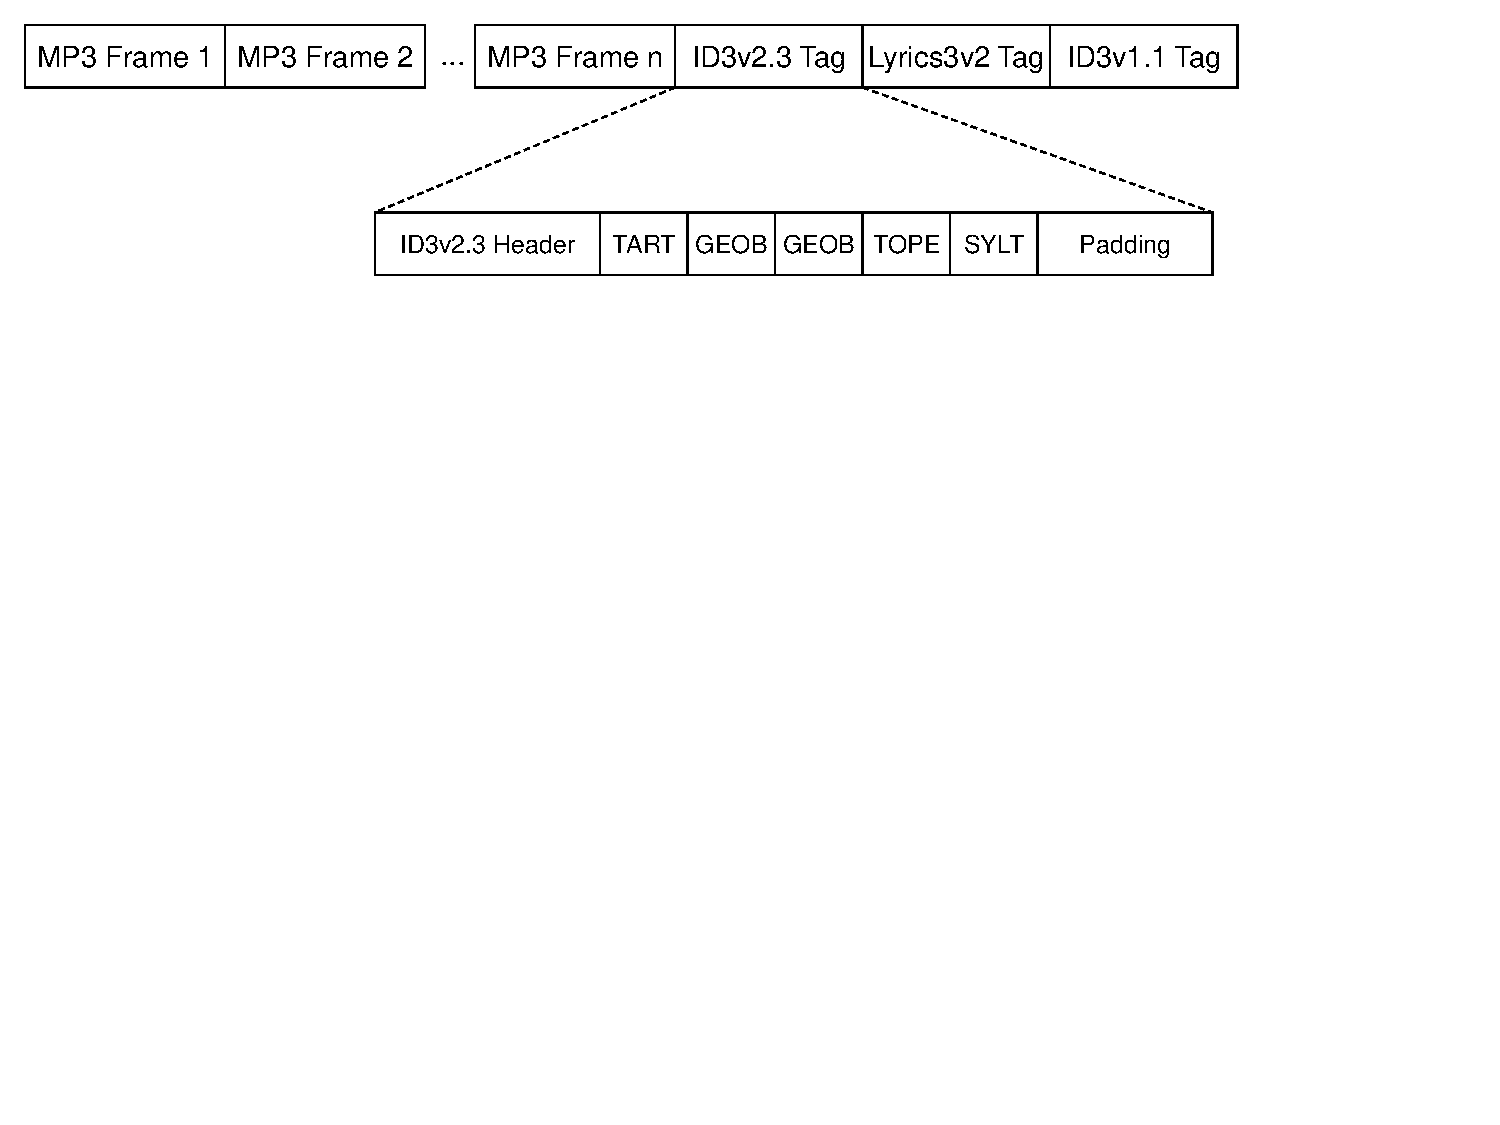
\includegraphics[width=1.00\textwidth]{figures/I_Example1.pdf}
\caption{Example 1: MP3 file with two tags}
\label{fig:Example1MP3filewithtwotags}
\end{figure}

The ID3v2.3 tag has several frames, including two \texttt{GEOB} frames. Furthermore, it has some padding within. Each of the MP3 frames corresponds to the MPEG-1 elementary stream audio format.

%-----------------------------------------------------------------------------------------------
%		Example 2: MP3 File with two ID3v2.4 Tags
%-----------------------------------------------------------------------------------------------

\section{Example 2: MP3 File with two ID3v2.4 Tags}
\label{sec:Example2MP3FileWithID3v23AndID3v11}

The following figure shows the second example, an MP3 file with two ID3v2.4 \TERMtag{}s, one at the beginning, the other one at the end of the file:

\begin{figure}[H]
\centering
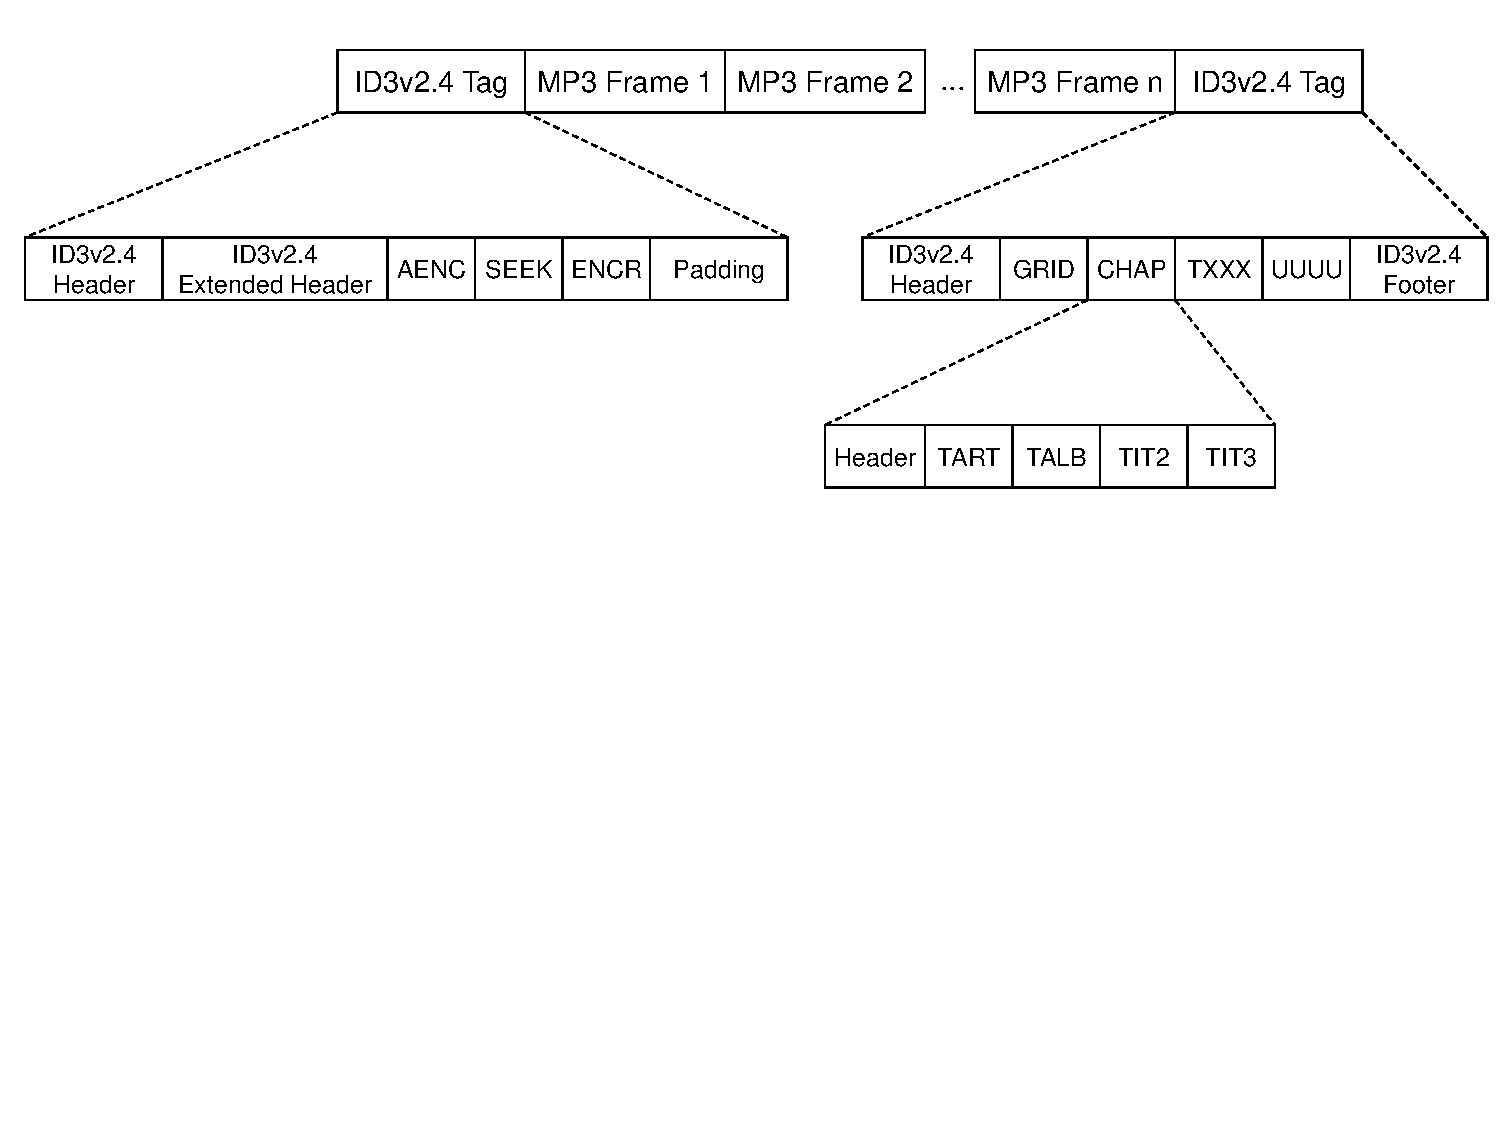
\includegraphics[width=1.00\textwidth]{figures/I_Example2.pdf}
\caption{Example 2: MP3 file with two ID3v2.4 tags}
\label{fig:Example1MP3filewithtwoID3tags}
\end{figure}

The two ID3v2.4 tags are virtually connected by a \texttt{SEEK} frame. Both have several specialties described in \cite{MC17}.

%-----------------------------------------------------------------------------------------------
%		Example 3: Ogg Bitstream with Theora and VorbisComment
%-----------------------------------------------------------------------------------------------

\section{Example 3: Ogg Bitstream with Theora and VorbisComment}
\label{sec:Example4MP3FileWithID3v23AndID3v11}

The following figure shows the fourth example, an Ogg bitstream that contains Theora payload data with a corresponding vorbis comment:

\begin{figure}[H]
\centering
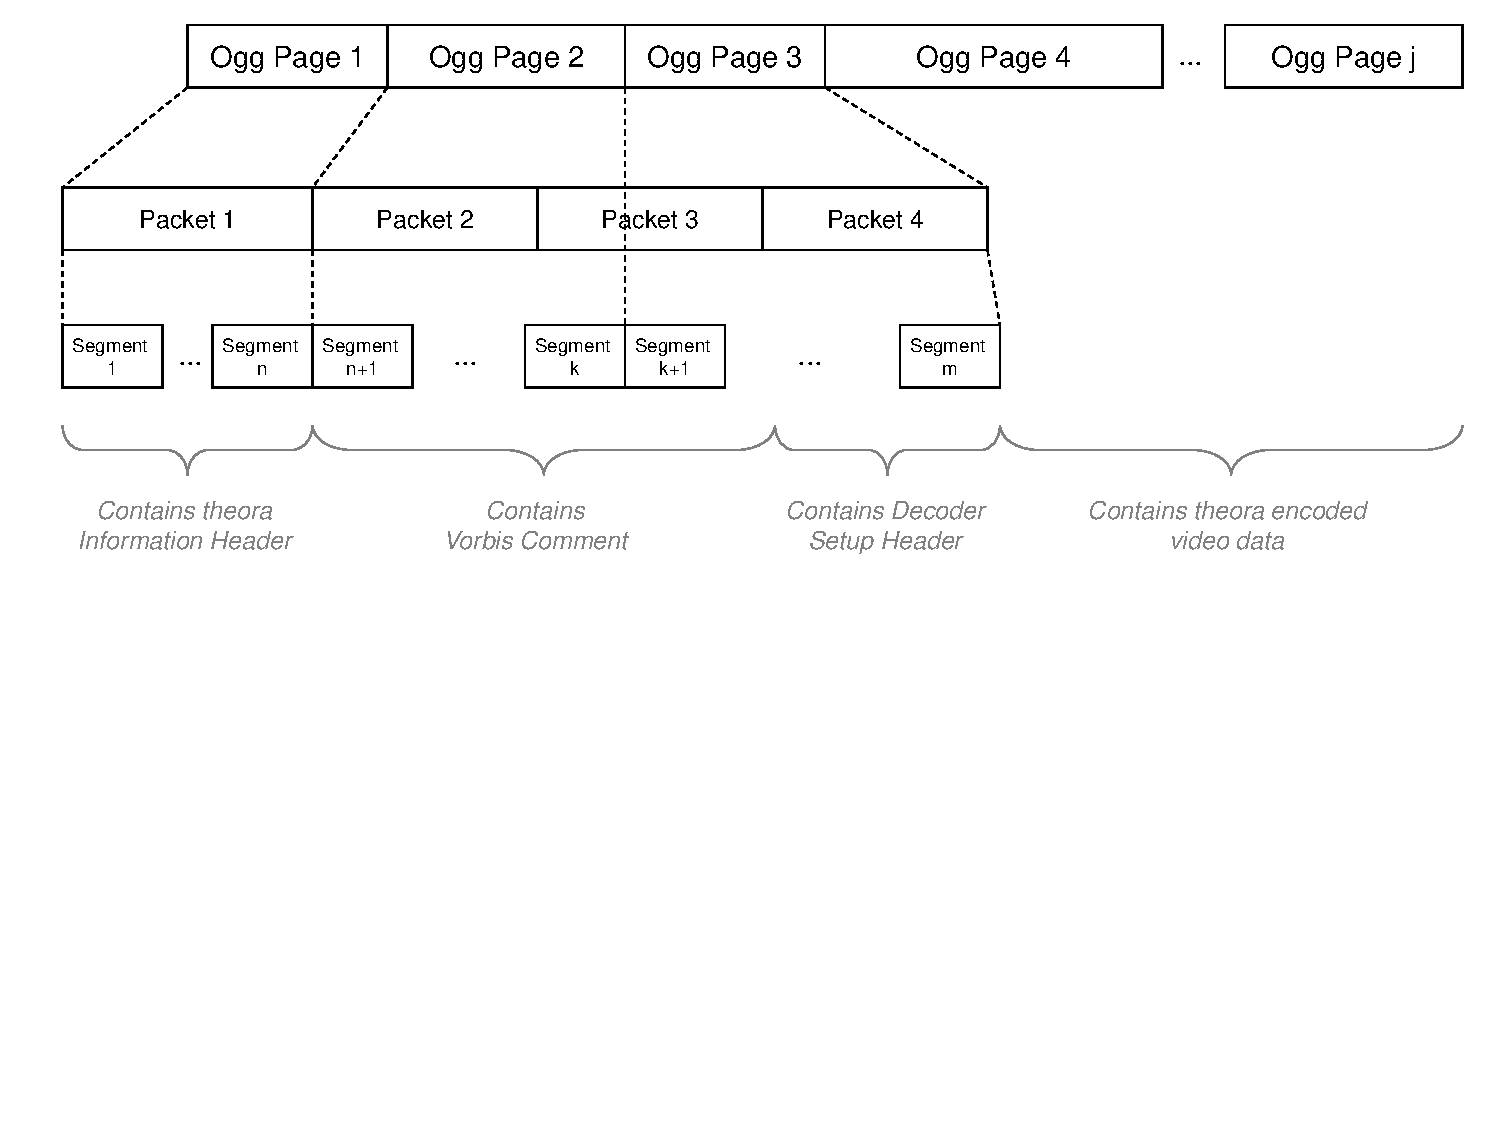
\includegraphics[width=1.00\textwidth]{figures/I_Example4.pdf}
\caption{Example 4: Ogg Bitstream with Theora and VorbisComment}
\label{fig:Example4MP3filewithtwoID3tags}
\end{figure}

The example is complex on first sight. In an Ogg bitstream, physical and logical structure are not necessarily the same. The physical structure is built by pages, packets and segments, while the logical structure is the structure of the wrapped data. We took theora video data as an example, but its basically arbitrary, as the codec does not really matter. What matters is where the Vorbis Comment, one of the supported data formats, is stored. This unfortunately depends on the embedded codec. In this example, the vorbis comment starts in the second page and spans over two packets. The second of these packets spans over two Ogg pages.

% %-----------------------------------------------------------------------------------------------
% %		Example 4: MP3 Media Stream with periodic ID3v2.3 Tags
% %-----------------------------------------------------------------------------------------------

% \section{Example 3: MP3 Media Stream with periodic ID3v2.3 Tags}
% \label{sec:Example3MP3FileWithID3v23AndID3v11}

% The following figure shows the third example, an MP3 media stream with wildly scattered or periodic ID3v2.3 \TERMtag{}s. The figure shows that start of listening to the stream may also be in the middle of an MP3 block:

% \begin{figure}[H]
% \centering
% 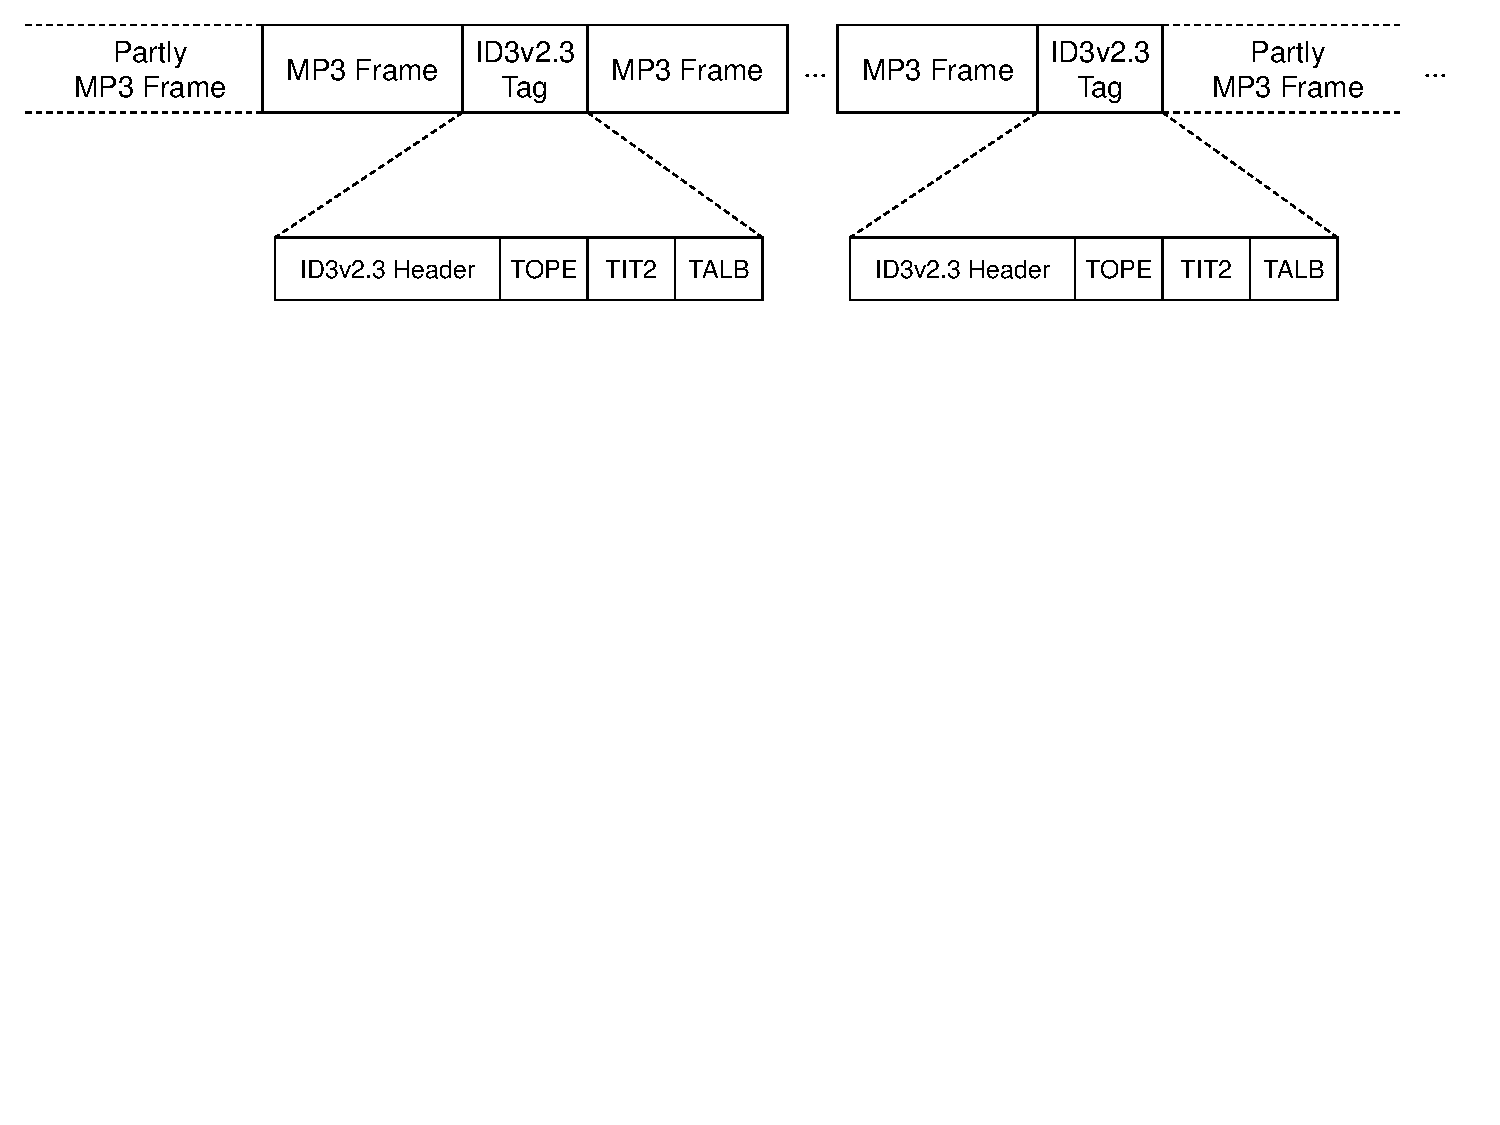
\includegraphics[width=1.00\textwidth]{figures/I_Example3.pdf}
% \caption{Example 3: MP3 Media Stream with periodic ID3v2.3 Tags}
% \label{fig:Example3MP3filewithtwoID3tags}
% \end{figure}

% %-----------------------------------------------------------------------------------------------
% %		Example 5: TIFF RGB image file
% %-----------------------------------------------------------------------------------------------

% \section{Example 5: TIFF RGB image file with Exif IFD}
% \label{sec:Example5MP3FileWithID3v23AndID3v11}

% An example RGB image TIFF file with an Exif IFD is modelled in the following figure:\footnote{The example is based on the figure of \cite{ExifSpec}, page 9.}

% \begin{figure}[H]
%\centering
%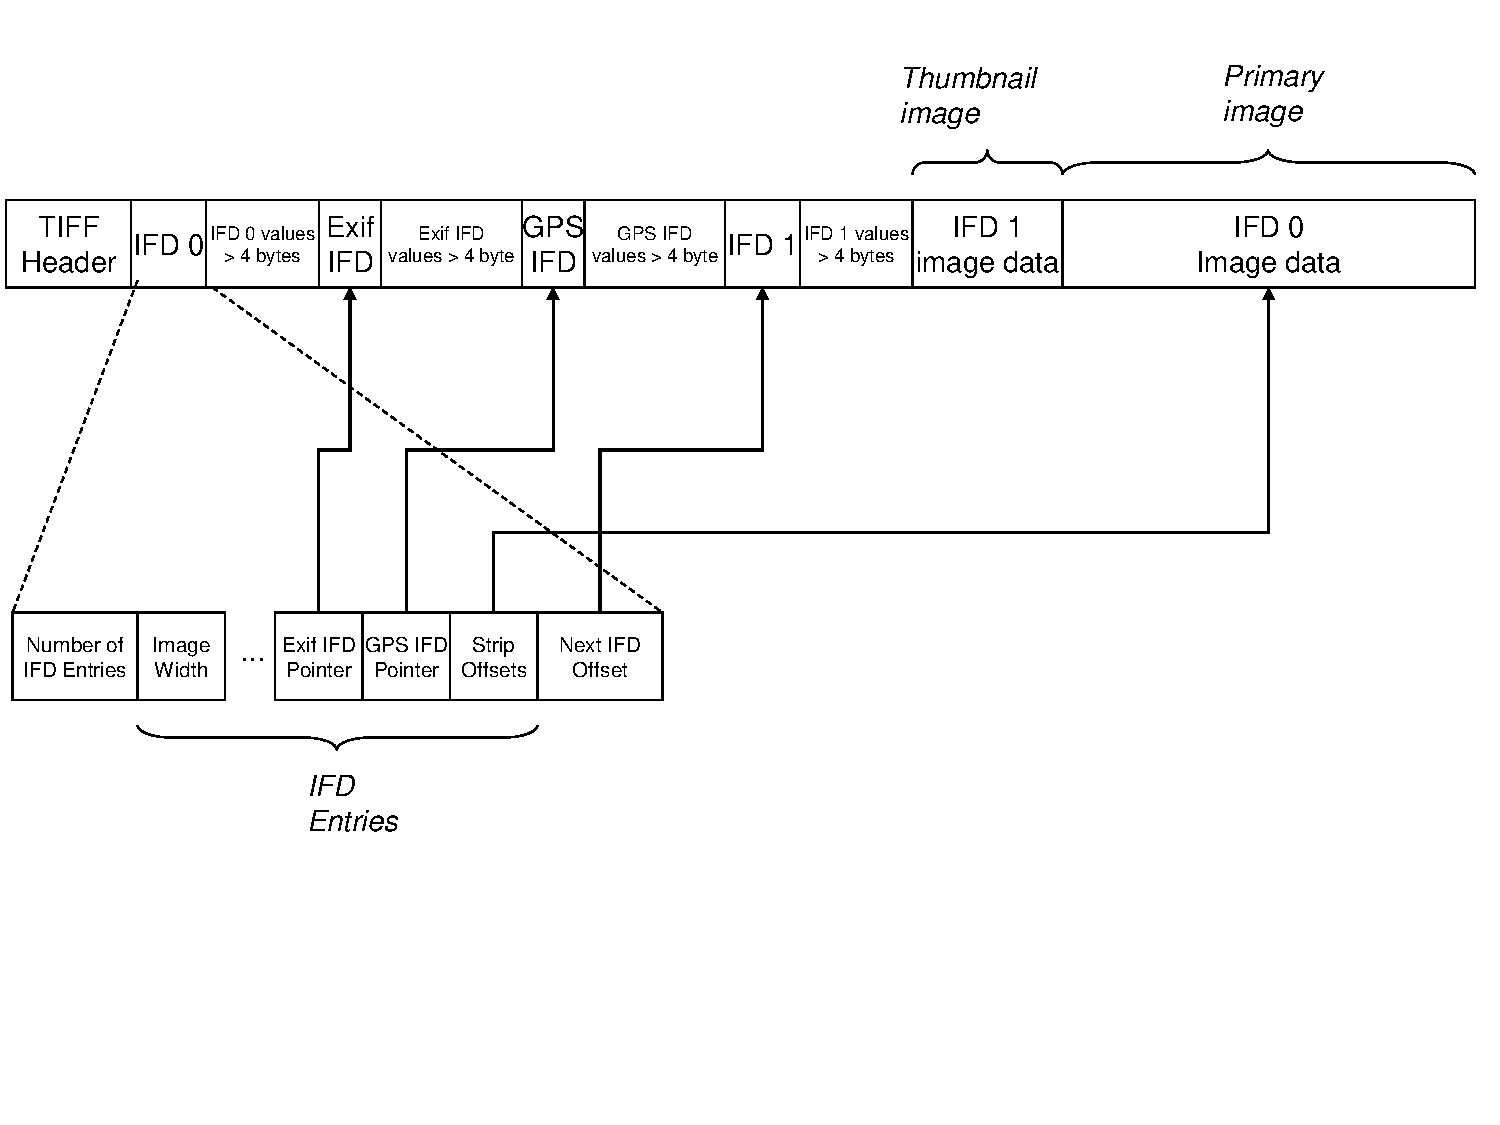
\includegraphics[width=1.00\textwidth]{figures/I_Example5.pdf}
%\caption{Example 5: TIFF RGB image file with Exif IFD}
%\label{fig:Example5MP3filewithtwoID3tags}
% \end{figure}

% Note that Exif is \emph{not a supported format} for \LibName{} currently. However, the presence of an Exif IFD must not be a problem for \LibName{}, of course.

% The example contains two image data parts, in this example stored after each other. The first image part is just a thumbnail image while the second one stores the real image data. The figure shows the pointered structure of the file as IFD fields often point to a byte offset in the file where the actual data is stored.

% %-----------------------------------------------------------------------------------------------
% %		Example 6: RIFF WAVE File
% %-----------------------------------------------------------------------------------------------

% \section{Example 6: RIFF WAVE File}
% \label{sec:Example6MP3FileWithID3v23AndID3v11}

% An example RIFF file with WAVE sound contents is shown in the following figure:

% \begin{figure}[H]
%\centering
%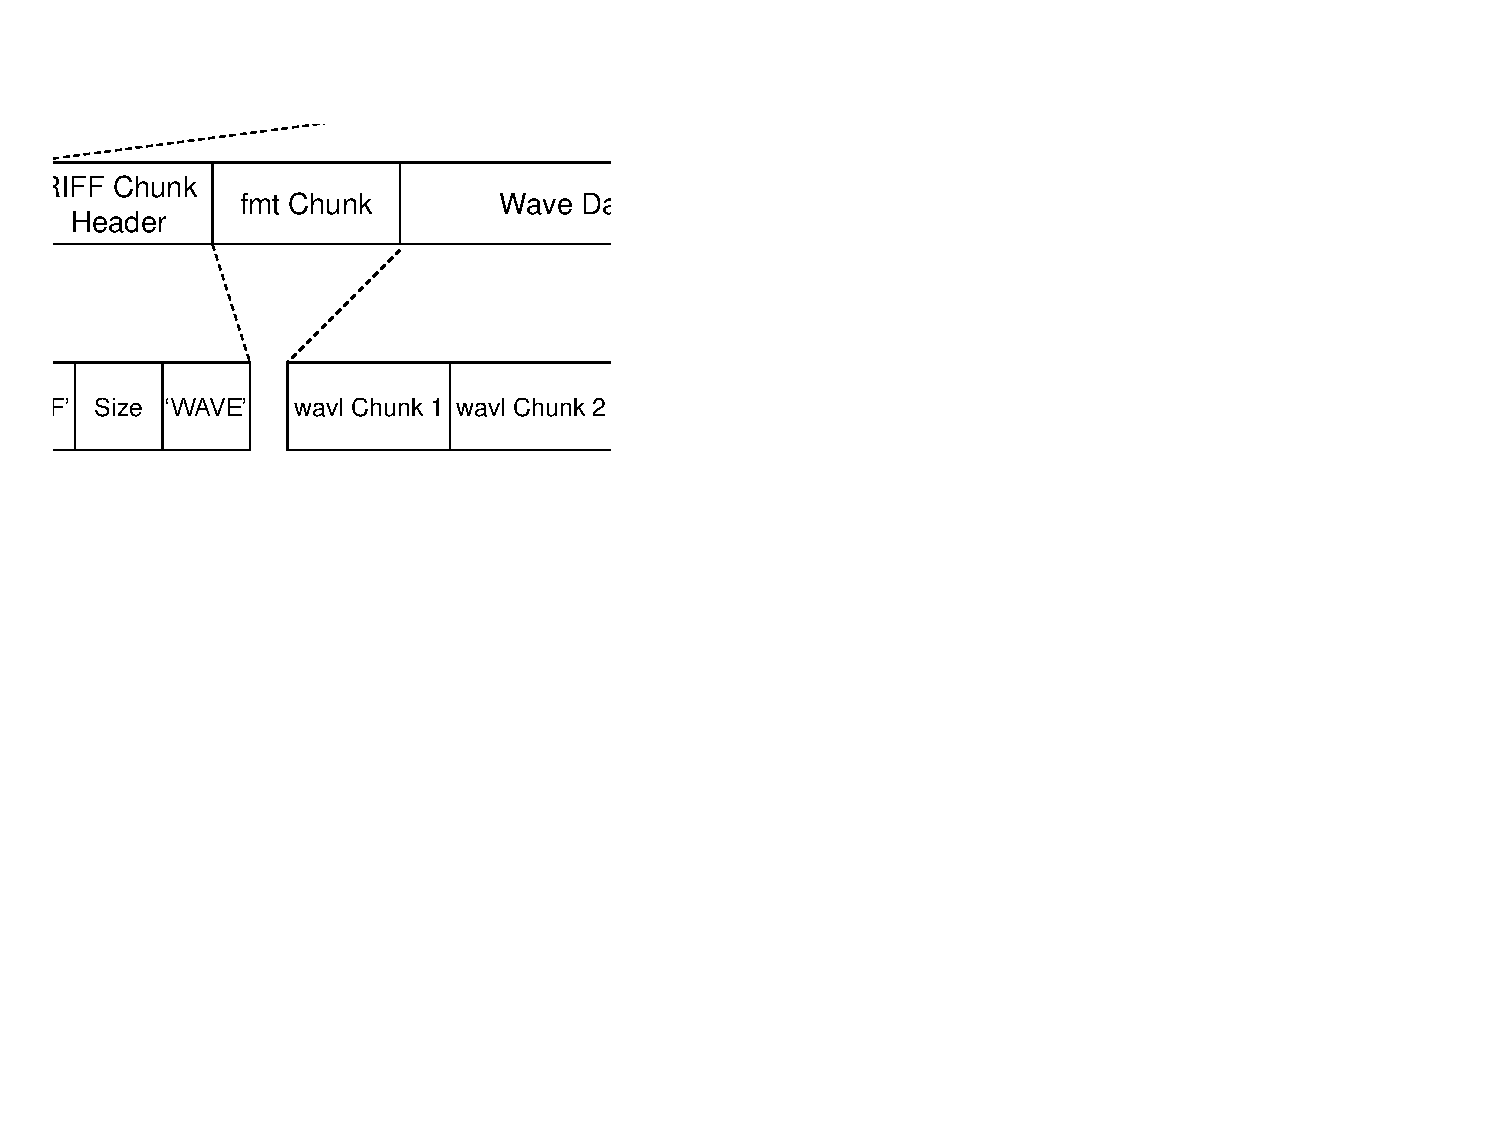
\includegraphics[width=1.00\textwidth]{figures/I_Example6.pdf}
%\caption{Example 6: RIFF WAVE File}
%\label{fig:Example6MP3filewithtwoID3tags}
% \end{figure}

% The top-level root chunk contains a fact chunk, a format chunk, a list of wave data chunks and finally a \texttt{LIST} info chunk in its payload. The \texttt{LIST} info chunk can be considered as \TERMtagBasic{}. It contains \texttt{INAM}, \texttt{IART} and \texttt{ICRD} sub-chunks.

% %-----------------------------------------------------------------------------------------------
% %		Example 7: QuickTime File
% %-----------------------------------------------------------------------------------------------

% \section{Example 7: QuickTime File}
% \label{sec:Example7MP3FileWithID3v23AndID3v11}

% An example QuickTime file is shown in the following figure:

% \begin{figure}[H]
%\centering
%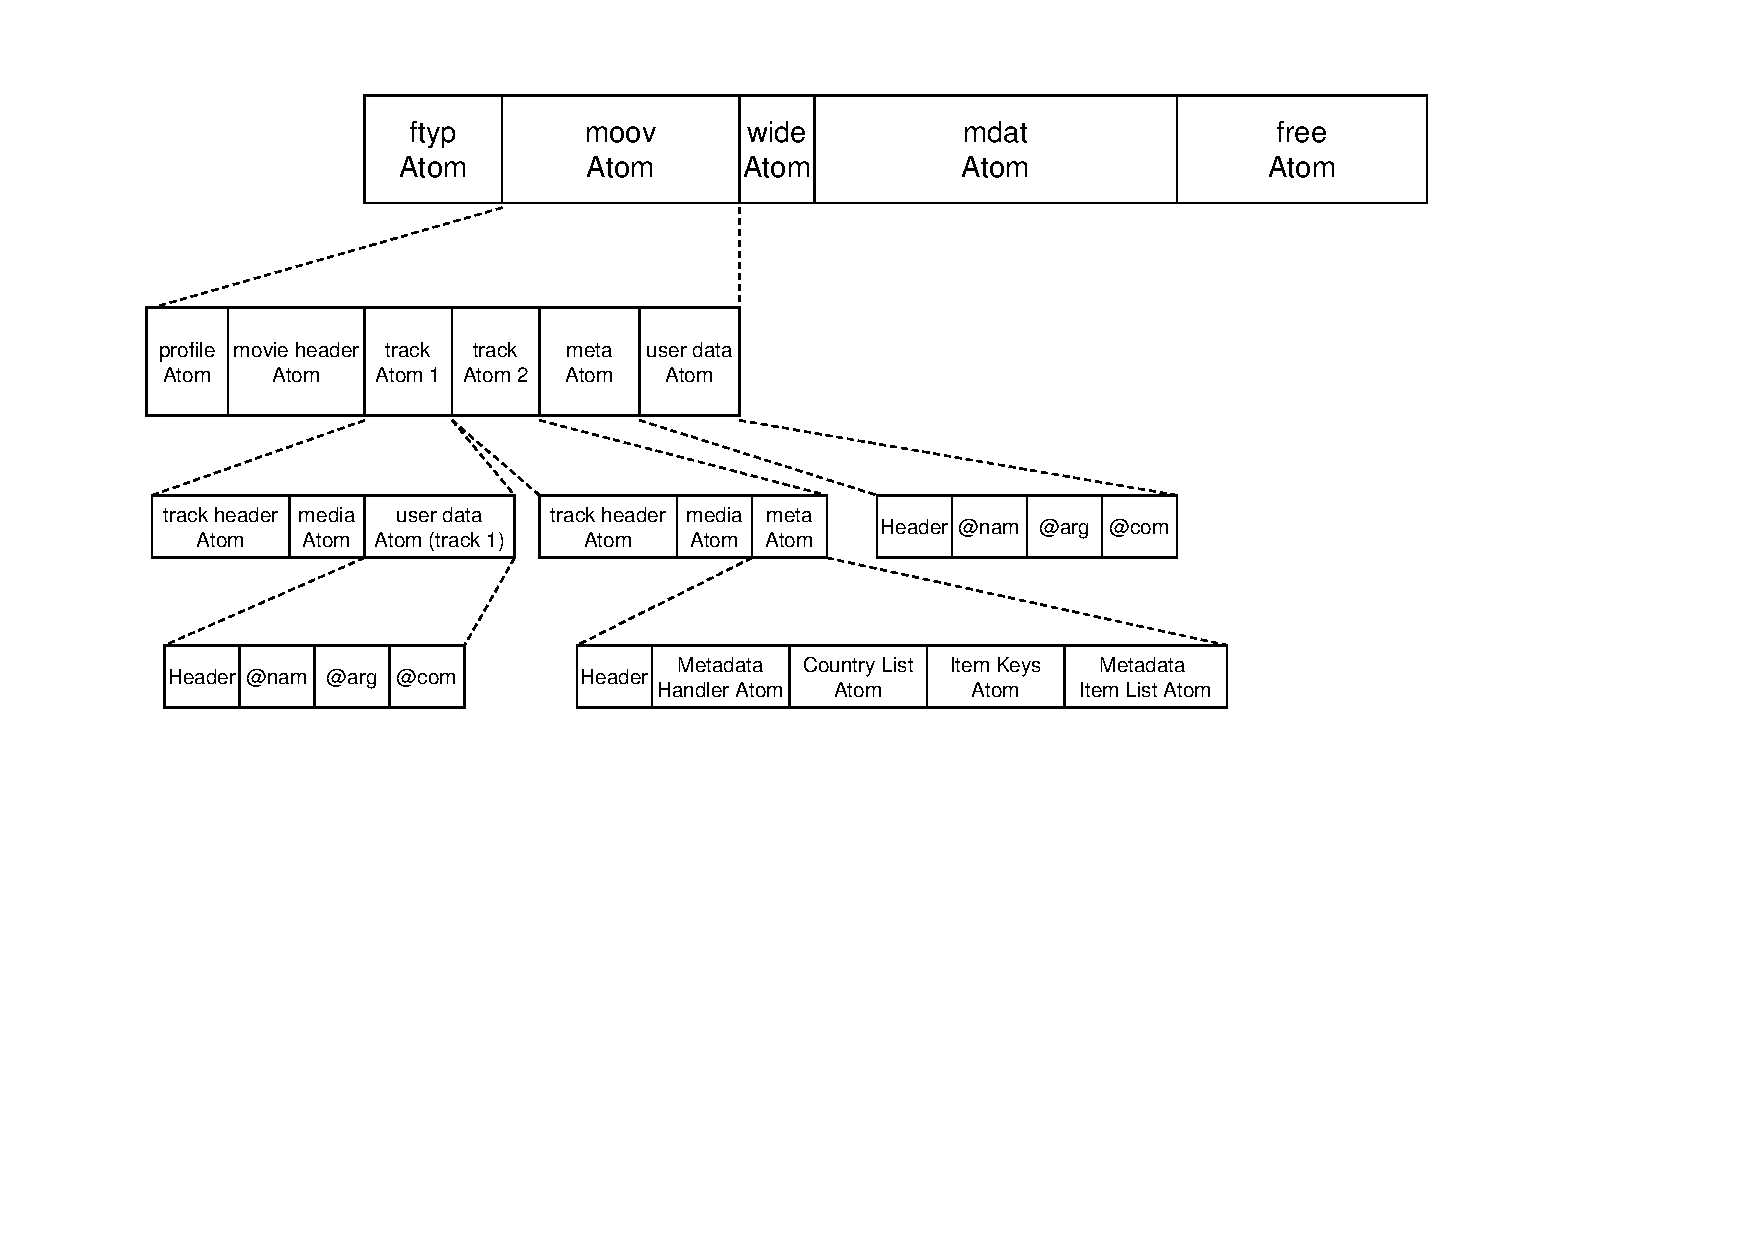
\includegraphics[width=1.00\textwidth]{figures/I_Example7.pdf}
%\caption{Example 7: QuickTime File}
%\label{fig:Example7MP3filewithtwoID3tags}
% \end{figure}

% A QuickTime file can easily get very complex. The example contains the \texttt{ftyp}, \texttt{moov}, \texttt{mdat} and \texttt{free} atoms as top-level atoms. The \texttt{mdat} atom contains the media data and is not further detailed in the example. It is preceded by a wide atom to enable easy extension to a header indicating more than $2^{32}$ bytes media atom size.

% The example defines two tracks in the movie atom. One of these contains a user data atom which contains key-value metadata. The other track contains the QuickTime \texttt{meta} atom also defining metadata, but in a different way.

% The example shows that the \texttt{moov} atom itself additionally contains a \texttt{meta} and user data atom describing the whole file.

% %-----------------------------------------------------------------------------------------------
% %		Example 8: Matroska File
% %-----------------------------------------------------------------------------------------------

% \section{Example 8: Matroska File}
% \label{sec:Example8MP3FileWithID3v23AndID3v11}

% An example Matroska file is shown in the following figure:

% \begin{figure}[H]
%\centering
%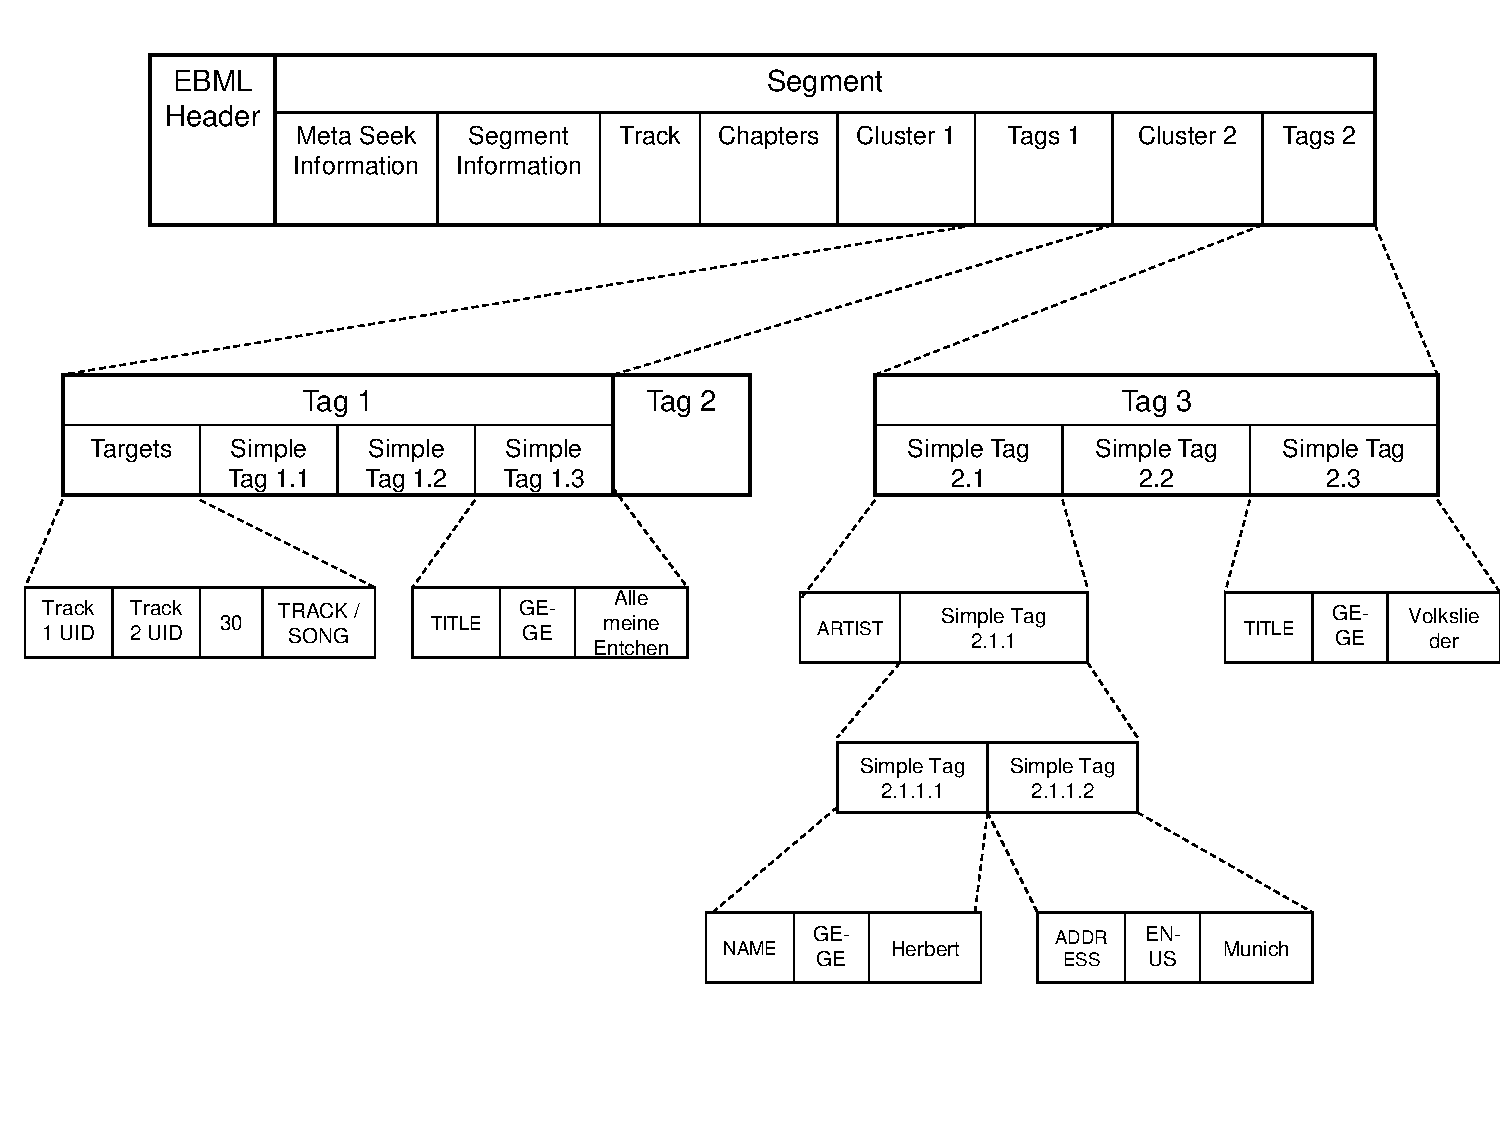
\includegraphics[width=1.00\textwidth]{figures/I_Example8.pdf}
%\caption{Example 8: Matroska File}
%\label{fig:Example8MP3filewithtwoID3tags}
% \end{figure}

% The example has two Cluster elements that store the actual media data. These are not further detailed in the example. The metadata in the example is complex: There are two top-level Tags elements, the first one contains two Tag elements, the second one only a single Tag element. Each of the Tag elements has child SimpleTag elements. The first Tag contains a Targets sub-element that points to two tracks of the file. Tag 3 only contains SimpleTags. However, the first SimpleTag contains nested SimpleTags.

% %-----------------------------------------------------------------------------------------------
% %		Example 9: Arbitrary XML
% %-----------------------------------------------------------------------------------------------

% \section{Example 9: Arbitrary XML}
% \label{sec:Example9MP3FileWithID3v23AndID3v11}

% \LibName{} is required to handle arbitrary XML data, too. The following short file is taken as an example:

% \begin{lstlisting}
% <?xml version="1.0" encoding="UTF-8"?>
% <!DOCTYPE ComponentConfiguration [ 

% <!ELEMENT ComponentDescriptor (Service+)>

% <!ATTLIST id NAME CDATA #REQUIRED>

% ]> 
% <cconf:ComponentConfiguration
% xmlns:cconf="www.easytag.de/XMLSchema_v1_0"
% 	xmlns:xsi="http://www.w3.org/2001/XMLSchema-instance"
% 	xsi:schemaLocation="www.easytag.de/XMLSchema_v1_0 ComponentConfiguration.xsd">
% 	<ComponentDescriptor id="a">
% 		<ProviderPath>bin/</ProviderPath>
% 		<Service>
% 			<Interface>de.je.registry.export.compdummies.a.export.TestInterfaceCompA1</Interface>
% 			<Provider>de.je.registry.compdummies.a.impl.TestImplCompA1</Provider>
% 		</Service>
% 		<Service>
% 			<Interface>de.je.registry.export.compdummies.a.export.TestInterfaceCompA2</Interface>
% 			<Provider>de.je.registry.compdummies.a.impl.TestImplCompA2</Provider>
% 		</Service>
% 	</ComponentDescriptor>
% 	<ComponentDescriptor id="b">
% 		<ProviderPath>bin/</ProviderPath>
% 		<Service>
% 			<Interface>de.je.registry.export.compdummies.b.export.TestInterfaceCompB1</Interface>
% 			<Provider>de.je.registry.compdummies.b.impl.TestImplCompB1</Provider>
% 		</Service>
% 	</ComponentDescriptor>
% 	<ComponentDescriptor id="c">
% 		<ProviderPath>bin/</ProviderPath>
% 		<Service>
% 			<Interface>de.je.registry.export.compdummies.c.export.TestInterfaceCompC1</Interface>
% 			<Provider>de.je.registry.compdummies.c.impl.TestImplCompC1</Provider>
% 		</Service>
% 	</ComponentDescriptor>
% 	<ComponentDescriptor id="d">
% 		<ProviderPath>bin/</ProviderPath>
% 		<Service>
% 			<Interface>de.je.registry.export.compdummies.d.export.XYZ</Interface>
% 			<Provider>de.je.registry.compdummies.d.impl.XYZImpl</Provider>
% 		</Service>
% 	</ComponentDescriptor>
% </cconf:ComponentConfiguration>
% \end{lstlisting}

% The example contains most XML elements: DTD, Elements, attributes, namespaces and of course the XML header.

% %-----------------------------------------------------------------------------------------------
% %		Example 10: Arbitrary XHTML with Meta Elements and RDFa
% %-----------------------------------------------------------------------------------------------

% \section{Example 10: Arbitrary XHTML with Meta Elements and RDFa}
% \label{sec:Example10MP3FileWithID3v23AndID3v11}

% \LibName{} is required to handle arbitrary XHTML data, and especially XHTML meta elements and embedded RDFa. All of this is contained in the following example:

% \begin{lstlisting}
% <?xml version="1.0" encoding="UTF-8"?>
% <!DOCTYPE html
%   PUBLIC "-//W3C//DTD XHTML 1.0 Transitional//EN"
%   "http://www.w3.org/TR/xhtml1/DTD/xhtml1-transitional.dtd">
% <html xmlns="http://www.w3.org/1999/xhtml"
%     version="XHTML+RDFa 1.0"
% 	 xmlns:biblio="http://example.org/"
%     xmlns:dc="http://purl.org/dc/elements/1.1/"
%     xmlns:cal="http://www.w3.org/2002/12/cal/ical#"
%  	 xmlns:foaf="http://xmlns.com/foaf/0.1/"
%     xml:lang="en"
%      profile="http://example.org/profil.html">
%   <head>
%     <title>Books by Marco Pierre White</title>
%     <!-- There is no about attribute here which means the predicate dc:creator with object (i.e. value) "Mark Birbeck" refers to the current document as a subject -->
%     <meta property="dc:creator" content="Mark Birbeck" />
%     <!-- Another example of a predicate that expresses a relationship "foaf:topic" to the specified URI. -->
%     <link rel="foaf:topic" href="http://www.formsPlayer.com/#us" />
% 	 <link rel="foaf:primaryTopic" href="#bbq" />
% 	<title>Beschreibung der Seite</title>
% 	<meta name="Typ" scheme="MIME-Type" content="image/svg+xml">
% 	<meta name="author" content="Anna Lyse">
% 	<meta http-equiv="expires" content="Sat , 01 Dec 2001 00:00:00 GMT">
% 	<meta name="keywords" lang="de" content="Ferien , Griechenland ,
% 		Sonnenschein">
% 	<meta name="keywords" lang="en-us" content="vacation , Greece , sunshine">
% 	<meta name="keywords" lang="en" content="holiday , Greece , sunshine">
% 	<meta name="keywords" lang="fr" content="vacances , Gr&egrave;ce , soleil">
% 	<meta http-equiv="content-type" content="text/html; charset=ISO-8859-1">
% 	<meta http-equiv="Content-Script-Type" content="text/javascript">

% 	<meta http-equiv="PICS-Label" content='(PICS-1.1 "http://www.gcf.org/v2.5"
% 		labels on "1994.11.05T08:15-0500"
% 		unti l "1995.12.31T23:59-0000"
% 		for "http://w3c.org/PICS/Overview.html"
% 		ratings ( suds 0.5 density 0 color/hue 1) ) '>
%   </head>
%   <body>
%     I think White's book
%     <!-- Here comes the first subject embedded in a span element. It refers to a specific datatype using typeof. It is described with the predicate dc:title whose object (i.e. value) is
%     the contents of the span element. -->
%     '<span about="urn:ISBN:0091808189" typeof="biblio:book"
%            property="dc:title">
%       Canteen Cuisine
%     </span>'
%     is well worth getting since although it's quite advanced stuff, he
%     makes it pretty easy to follow. You might also like
%     <!-- The second subject whose dc:description is given. -->
%     <span about="urn:ISBN:1596913614" typeof="biblio:book"
%           property="dc:description">
%       White's autobiography
%     </span>.
%     <!-- Another subject -->
%     <p about="#bbq" typeof="cal:Vevent">
%       I'm holding
%       <span property="cal:summary">
%         one last summer barbecue
%       </span>,
%       on
%       <!-- Here the object is not the content of the span attribute but the value of the "content" attribute -->
%       <span property="cal:dtstart" content="2007-09-16T16:00:00-05:00"
%             datatype="xsd:dateTime">
%         September 16th at 4pm
%       </span>.
%     </p>
% </body>
% </html>
% \end{lstlisting}

% The example is not real but constructed from various sources. It contains as much different elements as possible:
% \begin{itemize}
% 	\item Some meta elements with a @name attribute
% 	\item Some meta elements with a @http-equiv attribute
% 	\item A meta element containing PICS metadata. PICS is not directly supported in \Lib{}. However, the generic meta elements must be parsed correctly, no matter what they contain.
% 	\item Some meta elements using specific namespaces or profiles
% 	\item RDFa metadata
% \end{itemize}

% %-----------------------------------------------------------------------------------------------
% %		Example 11: An RDF/XML File
% %-----------------------------------------------------------------------------------------------

% \section{Example 11: An RDF/XML File}
% \label{sec:Example11MP3FileWithID3v23AndID3v11}

% \begin{lstlisting}
% <?xml version="1.0" encoding="UTF-8"?>
% <rdf:RDF xmlns:rdf="http://www.w3.org/1999/02/22-rdf-syntax-ns#"
%          xmlns:pcv="http://prismstandard.org/namespaces/pcv/1.0/"
%          xmlns:dc="http://purl.org/dc/elements/1.1/"
%          xml:base="http://travel.example.com/"
%          xmlns:s="http://example.org/students/vocab#"
%          xmlns:exterms="http://www.example.org/terms/">

%   <rdf:Description rdf:about="/2000/08/Corfu.jpg">
%     <dc:identifier rdf:resource="/content/2357845" />
%     <dc:creator>
%       <pcv:Descriptor rdf:about="/emp3845">
%         <pcv:label>John Peterson</pcv:label>
%       </pcv:Descriptor>
%     </dc:creator>
%     <dc:coverage>
%       <pcv:Descriptor
%           rdf:about="http://prismstandard.org/vocabs/ISO-3166/GR">
%         <pcv:label xml:lang="en">Greece</pcv:label>
%         <pcv:label xml:lang="fr">Grece</pcv:label>
%       </pcv:Descriptor>
%     </dc:coverage>
%   </rdf:Description>

%   <rdf:Description rdf:about="/2000/08/Corfu.jpg">
%     <dc:identifier rdf:resource="/content/2357845" />
%     <dc:creator>
%     	Michael
%     </dc:creator>
%   </rdf:Description>
  
%    <rdf:Description rdf:about="http://example.org/courses/6.001">
%       <s:students rdf:parseType="Collection">
%          <rdf:Description rdf:about="http://example.org/students/Amy"/>
%          <rdf:Description rdf:about="http://example.org/students/Mohamed"/>
%          <rdf:Description rdf:about="http://example.org/students/Johann"/>
%       </s:students>
%    </rdf:Description>

%   <rdf:Description rdf:about="http://www.example.com/2002/04/products#item10245">
%      <exterms:weight rdf:parseType="Resource">
%        <rdf:value rdf:datatype="&xsd;decimal">2.4</rdf:value>
%        <exterms:units rdf:resource="http://www.example.org/units/kilograms"/>
%      </exterms:weight>
%   </rdf:Description>

% </rdf:RDF>
% \end{lstlisting}

% The example contains several rdf:Description elements, even two referring to the same subject. We also have applications of the rdf:parseType, rdf:datatype and rdf:resource attributes. There are also some nested descriptions.

% %-----------------------------------------------------------------------------------------------
% %		Example 12: An XMP File
% %-----------------------------------------------------------------------------------------------

% \section{Example 12: An XMP File}
% \label{sec:Example12MP3FileWithID3v23AndID3v11}

% The following listing shows the XMP reference example:

% \begin{lstlisting}
% <?xpacket begin='?' id='W5M0MpCehiHzreSzNTczkc9d'?>
% <x:xmpmeta xmlns:x='adobe:ns:meta/' x:xmptk='XMPTk 2.8'>

% <rdf:RDF 
% 	xmlns:rdf='http://www.w3.org/1999/02/22-rdf-syntax-ns#' 
% 	xmlns:iX='http://ns.adobe.com/iX/1.0/'>

% 	<rdf:Description about=''
% 		xmlns:xmp='http://ns.adobe.com/xap/1.0/' 
% 		xmp:Author='Jane Doe'
% 		xmp:BaseURL='http://mydoc'
% 		xmp:CreateDate='2001-08-13T10:42:24Z'
% 		xmp:CreatorTool='Microsoft Visual C++ for Windows'
% 		xmp:Format='text/xml'
% 		xmp:MetadataDate='2001-08-13T10:42:24Z'
% 		xmp:ModifyDate='2001-08-13T11:02:13Z'
% 		xmp:Nickname='sample'>
    
% 		<xmp:Advisory>
% 			<rdf:Bag>    
%  				<rdf:li>http://purl.org/dc/elements/1.1/ format</rdf:li>
% 				<rdf:li>http://ns.adobe.com/xap/1.0/xap/g/ NumberOfColors</rdf:li>
% 				<rdf:li>http://ns.adobe.com/xap/1.0/xap/g/img/ Resolution/stRes:units</rdf:li>
% 			</rdf:Bag>
% 		</xmp:Advisory>
  
% 		<xmp:Authors>  
% 			<rdf:Seq>
% 				<rdf:li>Jane Doe</rdf:li>
% 				<rdf:li>John Doe</rdf:li>
% 				<rdf:li>Jack Doe</rdf:li>
% 			</rdf:Seq>
% 		</xmp:Authors>
% 		<xmp:Description>
% 			<rdf:Alt>
% 				<rdf:li xml:lang='en'>This document is a sample XML file</rdf:li>
% 				<rdf:li xml:lang='fr'>Ce document est un fichier d`exemple XML</rdf:li>
% 				<rdf:li xml:lang='de'>Dieses Dokument ist eine XML Beispieldatei</rdf:li>
% 			</rdf:Alt>
% 		</xmp:Description>
  
% 		<xmp:Keywords>
% 			<rdf:Bag>
% 				<rdf:li>XMP</rdf:li>
% 				<rdf:li>Core</rdf:li>
% 				<rdf:li>Schema</rdf:li>
% 				<rdf:li>sample</rdf:li>
% 			</rdf:Bag>
% 		</xmp:Keywords>
% 		<xmp:Locale>
% 			<rdf:Bag>
% 				<rdf:li>en</rdf:li>
% 				<rdf:li>fr</rdf:li>
% 				<rdf:li>de</rdf:li>
% 			</rdf:Bag>
% 		</xmp:Locale>
  
% 		<xmp:Title>
% 			<rdf:Alt>
% 				<rdf:li xml:lang='en'>XMP Core Schema Example</rdf:li>
% 				<rdf:li xml:lang='fr'>XMP Core Schema Exemple</rdf:li>
% 				<rdf:li xml:lang='de'>XMP Core Schema Beispiel</rdf:li>
% 			</rdf:Alt>
% 		</xmp:Title>
  
% 	</rdf:Description>

% </rdf:RDF>

% </x:xmpmeta>
% <?xpacket end='r'?>

% </top_level_element>
% \end{lstlisting}

%###############################################################################################
%###############################################################################################
%
%		File end
%
%###############################################################################################
%###############################################################################################


%%% Local Variables:
%%% mode: latex
%%% TeX-master: "jMetaDesignConcept"
%%% End: